\chapter{Đánh giá}

Hệ thống cuối đạt cả bốn kỳ vọng đã đăng ký trên một campaign mới, với p95 1,97 s. Điểm yếu chính là binary vô hại vẫn bị gắn cờ 89,5\%. Chương này đi theo thứ tự các câu hỏi nghiên cứu, sau phần phương pháp.

\section{Phương pháp}

\textbf{Đăng ký trước.} Mỗi lượt live và mỗi phân tích chính có một protocol JSON được commit vào git trước khi đọc bất kỳ dòng dữ liệu nào, ví dụ \texttt{final-\allowbreak{}system-\allowbreak{}confirmation-\allowbreak{}v1} hay \texttt{rule-\allowbreak{}integration-\allowbreak{}v1}. Protocol ghi kỳ vọng, định nghĩa chỉ số, luật chọn và code phân tích. Mọi sửa đổi sau đó là một amendment có giờ và lý do.

Kết quả được chia hai loại:

\begin{itemize}
\tightlist
\item
  \textbf{development:} trên dữ liệu đã nhìn khi phát triển;
\item
  \textbf{blind:} trên campaign mới, chưa dùng để chỉnh gì. Chỉ kết quả blind được dùng để kết luận cuối.
\end{itemize}

\textbf{Thiết kế trial.} Mỗi trial nhắm một replica và gồm ba đoạn 15 s liên tiếp trên cùng container:

\begin{enumerate}
\def\labelenumi{\arabic{enumi}.}
\tightlist
\item
  \textbf{Control idle:} không làm gì.
\item
  \textbf{Binary vô hại:} chạy qua cùng đường \texttt{kubectl\ exec} với tấn công, chỉ gọi \texttt{getpid} lặp lại. Đoạn này đo phần tín hiệu chỉ do có process mới.
\item
  \textbf{Tấn công:} một trong 5 kịch bản, lặp theo tốc độ đăng ký.
\end{enumerate}

\begin{longtable}[]{@{}>{\raggedright\arraybackslash}p{\dimexpr 0.389\linewidth-2\tabcolsep\relax}>{\raggedright\arraybackslash}p{\dimexpr 0.611\linewidth-2\tabcolsep\relax}@{}}
\toprule\noalign{}
Kịch bản & Hành vi \\
\midrule\noalign{}
\endhead
\bottomrule\noalign{}
\endlastfoot
\texttt{child\_\allowbreak{}ptrace\_\allowbreak{}handshake} & process con gọi \texttt{ptrace(PTRACE\_\allowbreak{}TRACEME)} \\
\texttt{invalid\_\allowbreak{}setns\_\allowbreak{}burst} & gọi \texttt{setns} với file descriptor -1, luôn thất bại \\
\texttt{execveat\_\allowbreak{}resolution\_\allowbreak{}probe} & gọi \texttt{execveat} tới một file không tồn tại, luôn thất bại \\
\texttt{anonymous\_\allowbreak{}mprotect\_\allowbreak{}churn} & đổi qua lại quyền đọc và đọc--ghi của một trang nhớ ẩn danh \\
\texttt{seccomp\_\allowbreak{}api\_\allowbreak{}probe} & gọi \texttt{seccomp} với mã thao tác không hợp lệ \\
\end{longtable}

Mọi thao tác chỉ ảnh hưởng chính process, hoặc chắc chắn thất bại trước khi đổi trạng thái của host.

\textbf{Quy mô.} 21 workload × 5 kịch bản × 3 tốc độ (6, 12, 24 lần/s) cho 315 trial của \textbf{tập chính}. Từ lượt thứ tư, campaign thêm tốc độ 1 và 3 lần/s để đo kẻ tấn công chậm, nên có 525 trial. Thứ tự trial được xáo bằng seed cố định, và tấn công chỉ bắt đầu sau pha chọn 90 phút.

\textbf{Chỉ số:}

\begin{itemize}
\tightlist
\item
  \textbf{Recall:} tỉ lệ trial tấn công có cảnh báo trong đoạn tấn công.
\item
  \textbf{Control dương:} tỉ lệ đoạn control idle có cảnh báo.
\item
  \textbf{Precision 1:1:} TP / (TP + control dương), vì mỗi trial có đúng một đoạn tấn công và một đoạn control. Tỉ lệ binary vô hại bị gắn cờ được báo riêng, không tính vào precision.
\item
  \textbf{Độ trễ:} từ sự kiện kernel đầu tiên của tấn công tới cuối cửa sổ cảnh báo đầu tiên. Đường tới người nhận qua Alertmanager được đo riêng ở mục 6.8.
\item
  \textbf{Gánh cảnh báo:} số đợt cảnh báo trên mỗi replica-giờ normal, ngoài các khoảng campaign. Một đợt gồm các cửa sổ báo của cùng container cách nhau dưới 15 s.
\end{itemize}

Khoảng tin cậy 95\% dùng Wilson cho tỉ lệ và bootstrap theo workload (10.000 lần) cho gánh cảnh báo và hiệu giữa hai cấu hình.

Có hai cách đếm dùng song song, chênh nhau vài trial:

\begin{itemize}
\tightlist
\item
  \textbf{cách của bộ điều phối campaign:} đếm tới lúc preview được ghi, ví dụ 308/310;
\item
  \textbf{cách so sánh các nhánh:} đếm trên bảng cửa sổ chung của mọi nhánh, ví dụ 313/315.
\end{itemize}

Mỗi bảng dưới đây ghi rõ nó dùng cách nào.

\textbf{Nhãn.} Nhãn là nhãn kỳ vọng theo thiết kế trial. 4.766 cảnh báo trên normal đã được review và không case nào có dấu hiệu độc hại, nhưng người review không độc lập với người thiết kế.

\section{RQ1: sáu lượt live}

\begingroup\footnotesize
\begin{longtable}[]{@{}>{\raggedright\arraybackslash}p{\dimexpr 0.233\linewidth-2\tabcolsep\relax}>{\raggedright\arraybackslash}p{\dimexpr 0.221\linewidth-2\tabcolsep\relax}>{\raggedright\arraybackslash}p{\dimexpr 0.125\linewidth-2\tabcolsep\relax}>{\raggedright\arraybackslash}p{\dimexpr 0.100\linewidth-2\tabcolsep\relax}>{\raggedright\arraybackslash}p{\dimexpr 0.115\linewidth-2\tabcolsep\relax}>{\raggedright\arraybackslash}p{\dimexpr 0.137\linewidth-2\tabcolsep\relax}>{\raggedright\arraybackslash}p{\dimexpr 0.069\linewidth-2\tabcolsep\relax}@{}}
\toprule\noalign{}
Lượt & Luật & Precision & Recall & Control dương & Binary vô hại bị gắn cờ & p95 (s) \\
\midrule\noalign{}
\endhead
\bottomrule\noalign{}
\endlastfoot
pulse-\allowbreak{}live-\allowbreak{}recalibrated & 1 cửa sổ, α×3 & 89,1\% & 92,8\% & 11,2\% & 80,7\% & 1,90 \\
pulse-\allowbreak{}stable-\allowbreak{}candidate & k2of2, α×10 & 92,2\% & 97,8\% & 8,4\% & 92,0\% & 1,85 \\
pulse-\allowbreak{}stable-\allowbreak{}refreshed & k2of2, α×10 + calibration mới & 96,0\% & 100,0\% & 4,2\% & 94,1\% & 2,26 \\
pulse-\allowbreak{}stable-\allowbreak{}confirm & CUSUM b3/h6 \texttt{cap} & 94,6\% & 100,0\% & 5,8\% & 95,1\% & 2,53 \\
pulse-\allowbreak{}peer-\allowbreak{}discount-\allowbreak{}confirm & k2of2 α×5 + chiết khấu replica 30 s & 98,7\% & 98,7\% & 1,3\% & 86,1\% & 2,88 \\
pulse-\allowbreak{}final-\allowbreak{}system-\allowbreak{}confirm (phần ML) & như trên & 99,4\% & 99,4\% & 0,6\% & 89,7\% & 2,38 \\
\end{longtable}
\endgroup

Tập chính, cách đếm của bộ điều phối campaign. Khoảng Wilson của từng ô nằm trong báo cáo kỹ thuật.

Bảng cho thấy ba bước tiến:

\begin{enumerate}
\def\labelenumi{\arabic{enumi}.}
\tightlist
\item
  \textbf{Xác nhận hai cửa sổ (k2of2)} hạ control từ 11,2\% xuống 8,4\% và đưa recall lên 97,8\%.
\item
  \textbf{Làm mới calibration} ngay trước lượt chạy đưa precision lên 96,0\%. Đây là lượt đầu đạt cả bốn kỳ vọng ở mức ≤ 3 s, nhưng gánh còn 6,74 đợt/replica-giờ.
\item
  \textbf{Chiết khấu theo replica} hạ control xuống 1,3\% và gánh xuống 1,69 đợt/replica-giờ.
\end{enumerate}

CUSUM \texttt{cap} không đạt ở lượt xác nhận của nó: control 5,8\% vượt ngưỡng 5\%. Vì vậy nó bị thay theo luật đã đăng ký.

\begin{figure}[htbp]
  \centering
  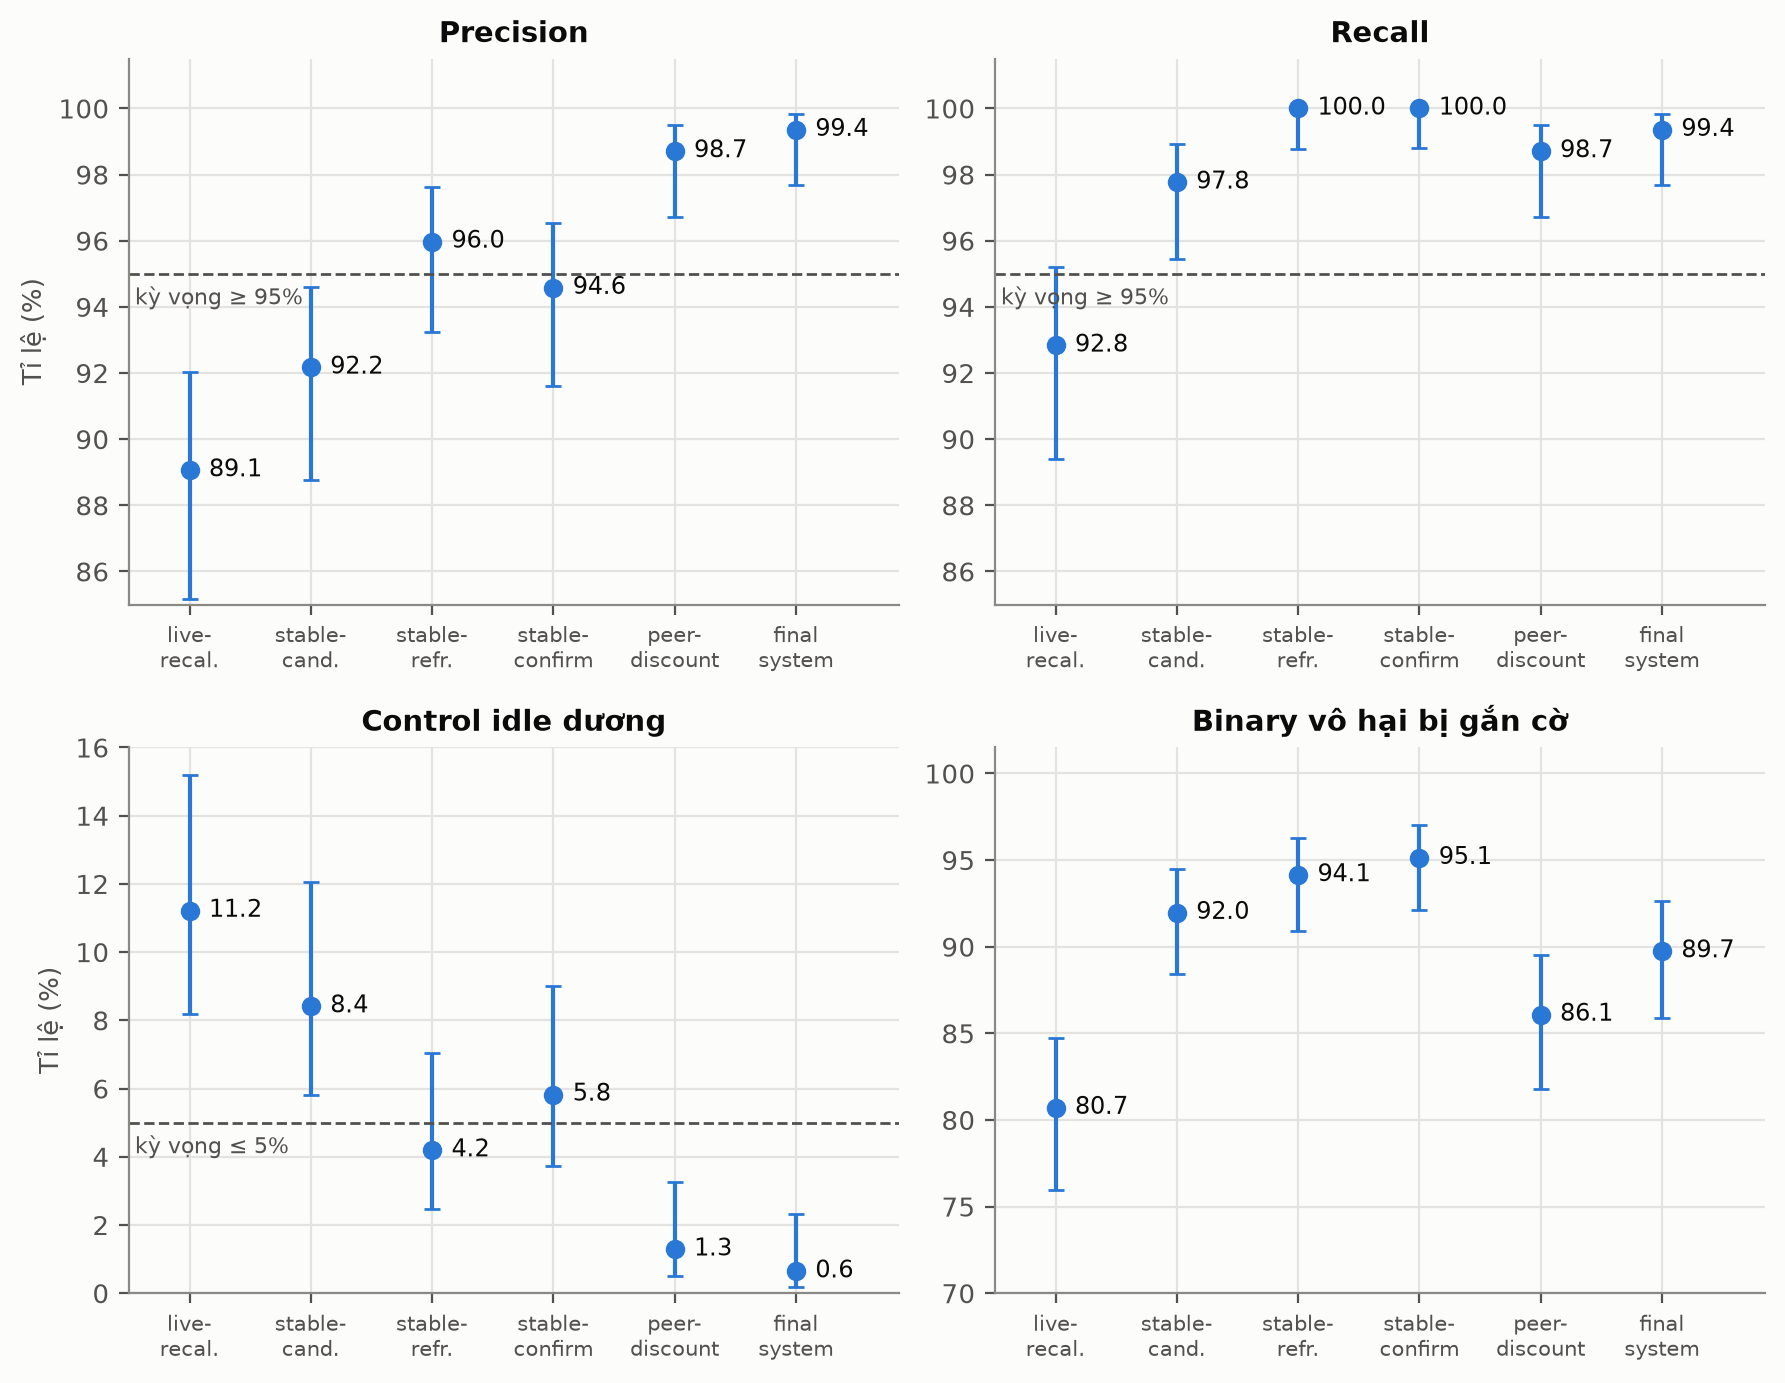
\includegraphics[width=0.85\linewidth]{live-runs-metrics-2x2.png}
  \caption{Precision, recall, control idle dương và binary vô hại bị gắn cờ qua 6 lượt live (phần ML, tập chính), khoảng tin cậy Wilson 95\%. Nhãn kỳ vọng.}
  \label{fig:live-runs-metrics}
\end{figure}

\section{Hệ thống cuối}

Lượt \texttt{pulse-\allowbreak{}final-\allowbreak{}system-\allowbreak{}confirm} chạy từ 25/10 22:05 đến khoảng 22:15 ngày 26/10, với 525 trial. ML được đóng băng từ lượt trước, còn tripwire chạy trong worker.

\begin{longtable}[]{@{}>{\raggedright\arraybackslash}p{\dimexpr 0.396\linewidth-2\tabcolsep\relax}>{\raggedright\arraybackslash}p{\dimexpr 0.198\linewidth-2\tabcolsep\relax}>{\raggedright\arraybackslash}p{\dimexpr 0.309\linewidth-2\tabcolsep\relax}>{\raggedright\arraybackslash}p{\dimexpr 0.097\linewidth-2\tabcolsep\relax}@{}}
\toprule\noalign{}
Chỉ số (tập chính, cách so sánh nhánh) & Kỳ vọng & ML + tripwire {[}CI 95\%{]} & Chỉ ML \\
\midrule\noalign{}
\endhead
\bottomrule\noalign{}
\endlastfoot
Recall & ≥ 95\% & 99,4\% (313/315) {[}97,7; 99,8{]} & 99,4\% \\
Precision & ≥ 95\% & 99,4\% {[}97,7; 99,8{]} & 99,4\% \\
Control dương & ≤ 5\% & 0,6\% (2/314) {[}0,2; 2,3{]} & 0,6\% \\
p95 kernel → cảnh báo đầu tiên & ≤ 3 s, ưu tiên \textless{} 2 s & 1,97 s & 2,25 s \\
Binary vô hại bị gắn cờ & báo kèm & 89,5\% (282/315) & 89,5\% \\
\end{longtable}

Recall, precision và control của hai cột trùng nhau theo định nghĩa, không phải do trùng dữ liệu với lượt khác:

\begin{itemize}
\tightlist
\item
  hệ thống là “ML hoặc tripwire”, nên không bao giờ kém ML;
\item
  ở tập chính, mọi trial mà tripwire bắt thì ML cũng bắt;
\item
  tripwire không gắn cờ control nào và không gắn cờ binary vô hại nào.
\end{itemize}

Tripwire đóng góp ở ba chỗ:

\begin{itemize}
\tightlist
\item
  \textbf{Độ trễ:} p95 nhanh hơn, hiệu nằm trong khoảng 0,02--0,85 s (CI).
\item
  \textbf{Recall trên mọi tốc độ:} tăng từ 93,5\% lên 96,4\%.
\item
  \textbf{Gánh cảnh báo:} trên 849,5 replica-giờ normal, ML có 1,50 đợt/replica-giờ và hệ thống có 1,55. Hiệu +0,049 {[}+0,005; +0,124{]} thấp hơn ngưỡng đăng ký 0,25, nên điều kiện “tripwire thêm rất ít gánh” đạt.
\end{itemize}

Tripwire đứng một mình có recall 60,0\%, vì nó không bắt \texttt{mprotect} và \texttt{seccomp}. P95 của nó là 0,77 s, control 0\%, gánh 0,062 đợt/replica-giờ.

\textbf{Kiểm cài đặt.} Hai bản khớp nhau hoàn toàn:

\begin{itemize}
\tightlist
\item
  tripwire live và tripwire tính lại offline cùng xét 10.417.205 cửa sổ, cùng báo 8.482 cửa sổ, và không lệch cửa sổ nào;
\item
  preview ML live khớp luật tính lại offline ở 99,9999\% cửa sổ.
\end{itemize}

Chênh lệch nhỏ của ML đúng chiều hỏng đã thiết kế: cửa sổ của peer tới muộn thì chiết khấu ít đi, nên live báo nhiều hơn.

\textbf{ML lặp lại.} Theo cách đếm của bộ điều phối, phần ML đạt recall 99,4\% (308/310), precision 99,4\%, control 0,6\% (2/311), p95 2,38 s. Kết quả này xác nhận lại lượt trước trên một campaign mới.

\begin{figure}[htbp]
  \centering
  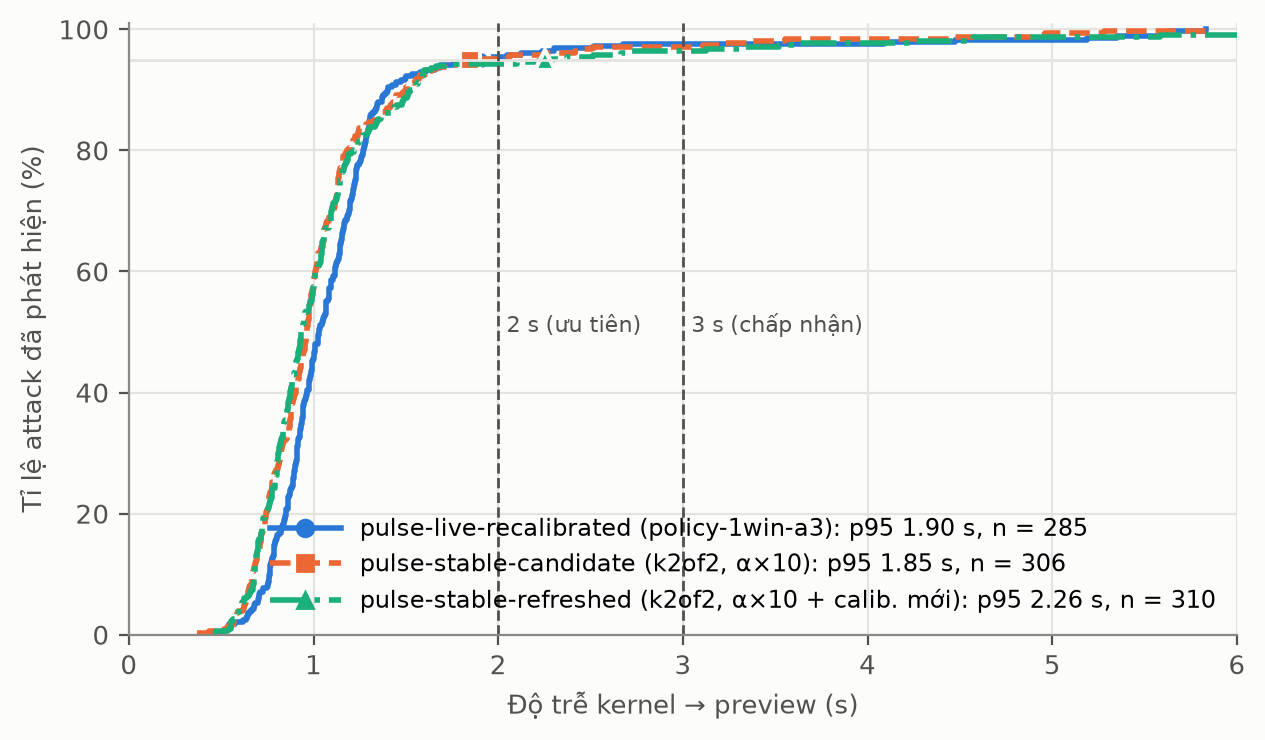
\includegraphics[width=\linewidth]{live-latency-cdf.png}
  \caption{Phân bố độ trễ kernel → preview của các attack được phát hiện, bốn lượt live gần nhất (phần ML, tập chính).}
  \label{fig:live-latency-cdf}
\end{figure}

\section{Kẻ tấn công chậm}

\begin{longtable}[]{@{}ll@{}}
\toprule\noalign{}
Tốc độ (lần/s) & Recall của ML, lượt cuối \\
\midrule\noalign{}
\endhead
\bottomrule\noalign{}
\endlastfoot
1 & 79,0\% (83/105) \\
3 & 90,2\% (92/102) \\
6 & 99,0\% \\
12 & 99,0\% \\
24 & 100\% \\
\end{longtable}

Recall giảm rõ ở 1/s. Chiết khấu theo replica đổi một phần recall ở tấn công chậm lấy control thấp hơn. Ở lượt \texttt{pulse-\allowbreak{}stable-\allowbreak{}confirm}, khi chưa có chiết khấu, recall ở 1/s là 93,1\%. Lý do là cửa sổ của tấn công chậm có ít syscall lạ hơn, nên dễ trùng với hành vi mà các replica khác vẫn có trong 30 s.

\section{RQ2: syscall và nhóm feature nào mang tín hiệu}

Bộ \texttt{base29} được giữ nguyên: không cấu hình thay thế nào tốt hơn có ý nghĩa thống kê. Thí nghiệm fit 11 cấu hình feature đúng như Pulse (21 workload × 11 cấu hình × 3 seed = 693 model). Các cấu hình chỉ khác nhau ở phần syscall tường minh, và được so ở cùng ngân sách cảnh báo với bootstrap theo workload.

\begin{longtable}[]{@{}>{\raggedright\arraybackslash}p{\dimexpr 0.343\linewidth-2\tabcolsep\relax}>{\raggedright\arraybackslash}p{\dimexpr 0.483\linewidth-2\tabcolsep\relax}>{\raggedright\arraybackslash}p{\dimexpr 0.175\linewidth-2\tabcolsep\relax}@{}}
\toprule\noalign{}
Thay đổi so với base29 & Kết quả & Quyết định \\
\midrule\noalign{}
\endhead
\bottomrule\noalign{}
\endlastfoot
Bỏ cặp \texttt{execve}/\texttt{execveat} & Recall −6,7 đến −10,6 điểm, CI loại trừ 0; toàn bộ mức giảm nằm ở kịch bản \texttt{execveat} (100\% xuống 49--66\%) & Giữ \\
Thêm syscall theo tần suất (top-8/16/32) & Không tăng recall; p95 2,9--3,1 s so với 2,3 s & Không thêm \\
Thêm 15 syscall bảo mật hiếm & Chênh recall −0,4 đến +0,3 điểm, CI chứa 0 & Không thêm \\
Mọi ID syscall (\textasciitilde300 feature) & Recall +6--8 điểm ở ngân sách rộng, nhưng binary vô hại bị gắn cờ 96--100\%; p95 5,0 s & Không dùng \\
Bỏ nhánh support & Recall −28,2 {[}−42,5; −15,2{]} điểm; p95 chậm thêm 1,1--1,6 s & Giữ \\
Bỏ nhánh tree & Recall −5,2 {[}−10,6; −1,1{]} điểm ở ngân sách chặt & Giữ \\
Chỉ giữ bin, bỏ kênh syscall tường minh & Recall −13 điểm & Giữ kênh tường minh \\
Bỏ 5 feature tổng hợp & p95 chậm thêm 0,26--0,35 s & Giữ \\
\end{longtable}

Kết luận không đổi khi kiểm lại dưới k2of2 và dưới CUSUM. Bảy syscall hiếm (\texttt{ptrace}, \texttt{setns}, \texttt{execveat}, \texttt{mount}, \texttt{unshare}, \texttt{pivot\_\allowbreak{}root}, \texttt{recvmmsg}) bằng 0 trên 185 triệu lượt gọi normal. Vì vậy chúng mang tín hiệu tấn công mà không làm tăng báo nhầm.

Hai kịch bản dùng syscall phổ biến (\texttt{mprotect}, \texttt{seccomp}) là điểm yếu chung của mọi bộ syscall, với recall 70--83\% ở ngân sách chặt. Đổi bộ syscall không sửa được điểm yếu này.

\textbf{Giới hạn:} đây là kết quả development, và theo luật protocol thì kết quả chính thức là \emph{inconclusive}, vì không cấu hình nào đạt ngân sách 0,1 đợt/giờ. Các so sánh trên được làm ở ngân sách 1, 5 và 18 đợt/giờ.

\begin{figure}[htbp]
  \centering
  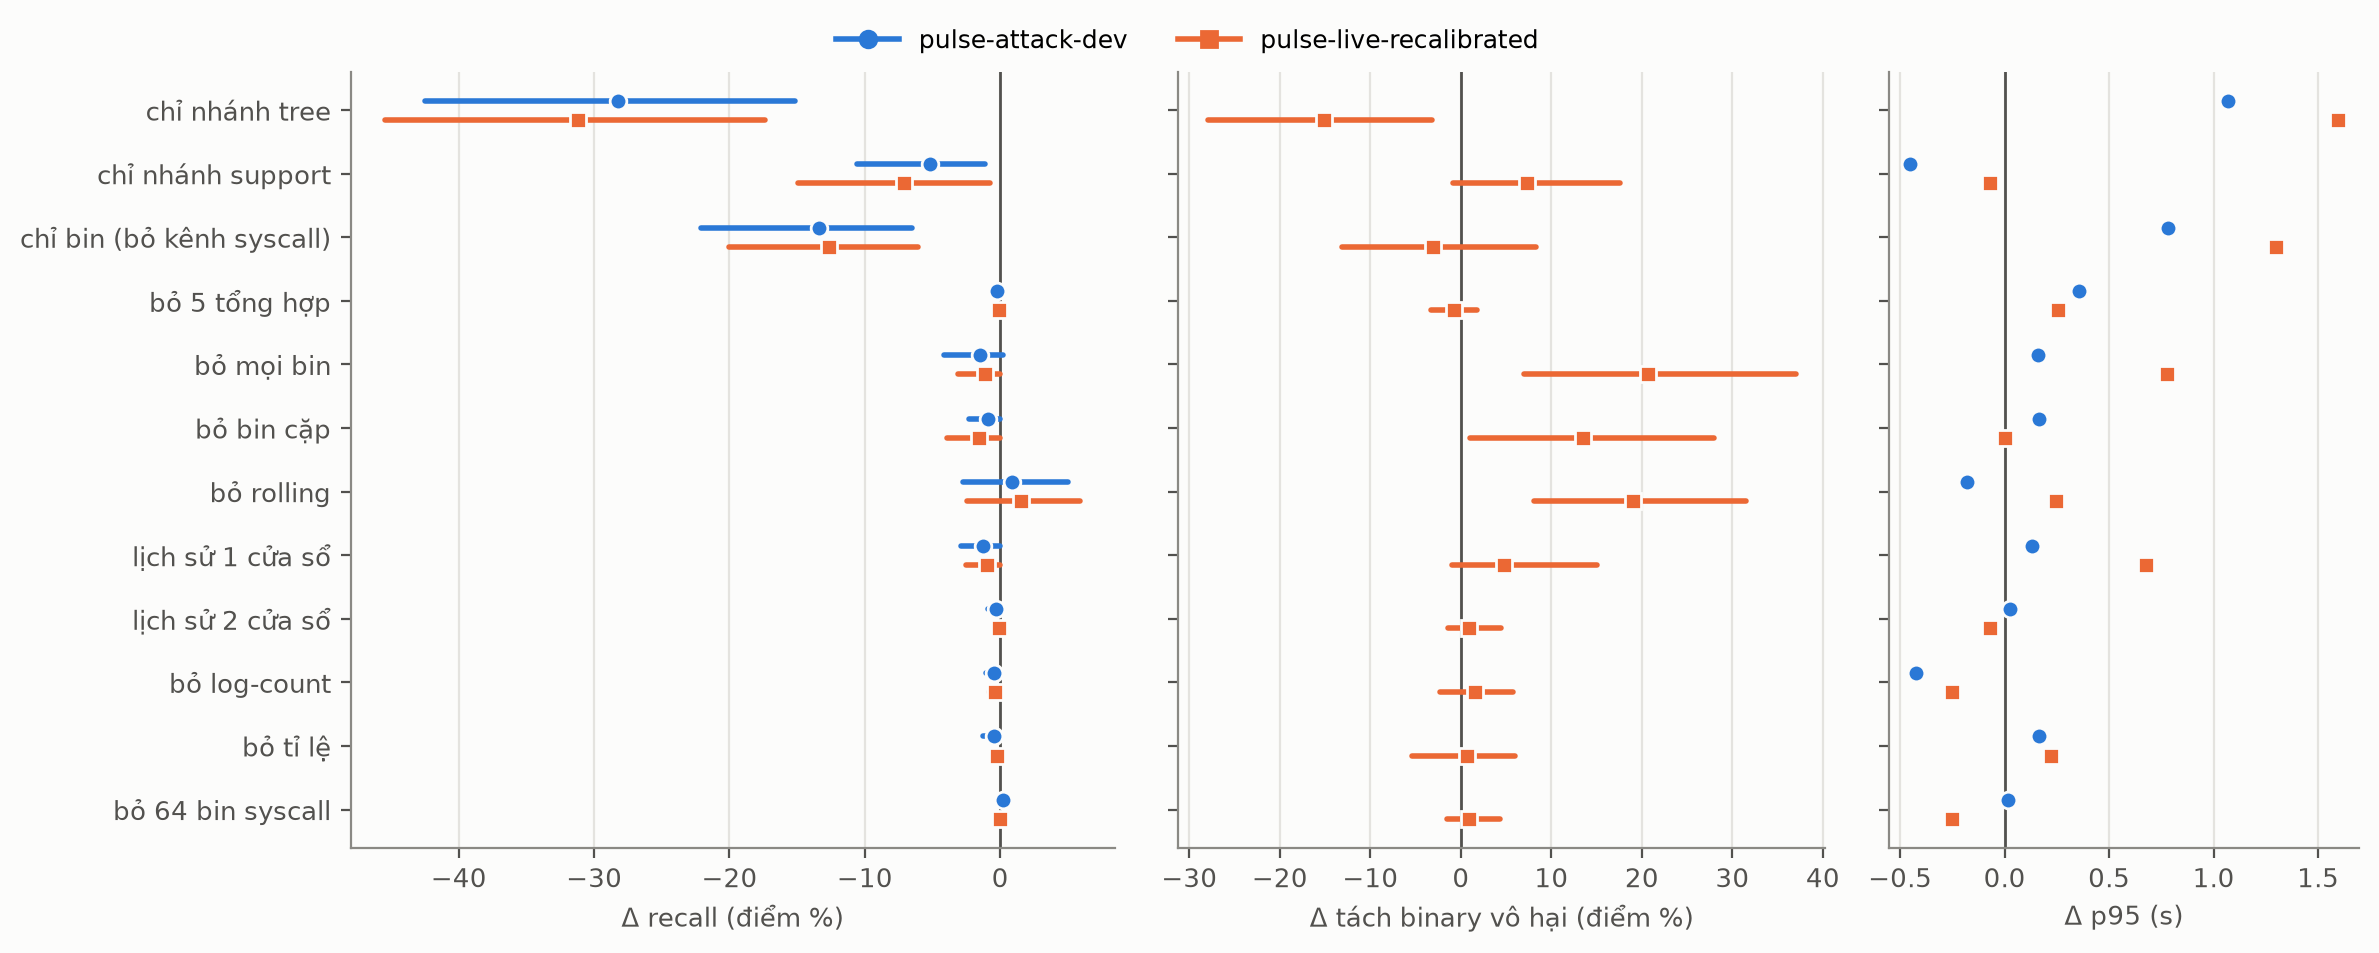
\includegraphics[width=\linewidth]{feature-groups.png}
  \caption{Thay đổi so với base29 khi bỏ một nhóm feature hoặc một nhánh p-value: hiệu recall, hiệu tách binary vô hại (CI bootstrap 95\% theo workload) và hiệu p95. Holdout chính, k2of2, ngân sách 1 (development).}
  \label{fig:feature-groups}
\end{figure}

\section{RQ4: có và không có luật}

Không luật nào tăng recall ở tập chính. ML + tripwire là cách gắn luật duy nhất giữ mọi chỉ số của ML, lại nhanh hơn và gần như không thêm gánh. So sánh chạy trên dữ liệu blind của \texttt{pulse-\allowbreak{}peer-\allowbreak{}discount-\allowbreak{}confirm}, với một khoảng normal chung 706,8 replica-giờ cho mọi nhánh.

\begingroup\footnotesize
\begin{longtable}[]{@{}>{\raggedright\arraybackslash}p{\dimexpr 0.166\linewidth-2\tabcolsep\relax}>{\raggedright\arraybackslash}p{\dimexpr 0.087\linewidth-2\tabcolsep\relax}>{\raggedright\arraybackslash}p{\dimexpr 0.136\linewidth-2\tabcolsep\relax}>{\raggedright\arraybackslash}p{\dimexpr 0.100\linewidth-2\tabcolsep\relax}>{\raggedright\arraybackslash}p{\dimexpr 0.125\linewidth-2\tabcolsep\relax}>{\raggedright\arraybackslash}p{\dimexpr 0.072\linewidth-2\tabcolsep\relax}>{\raggedright\arraybackslash}p{\dimexpr 0.134\linewidth-2\tabcolsep\relax}>{\raggedright\arraybackslash}p{\dimexpr 0.180\linewidth-2\tabcolsep\relax}@{}}
\toprule\noalign{}
Nhánh & Recall & Recall mọi tốc độ & Control & Precision & p95 (s) & Đợt/replica-giờ & Δ đợt so với A {[}CI{]} \\
\midrule\noalign{}
\endhead
\bottomrule\noalign{}
\endlastfoot
A: chỉ ML & 98,7\% & 94,5\% & 1,3\% & 98,7\% & 2,91 & 1,42 & --- \\
B1: ML + Falco & 98,7\% & 95,2\% & 2,9\% & 97,2\% & 2,48 & 2,54 & +1,120 {[}0,000; 3,252{]} \\
B2: ML + tripwire & 98,7\% & 96,6\% & 1,6\% & 98,4\% & 2,44 & 1,48 & +0,066 {[}0,020; 0,133{]} \\
B3: ML rồi lọc probe & 98,7\% & 94,5\% & 1,3\% & 98,7\% & 5,90 & 1,09 & −0,330 {[}−0,751; −0,092{]} \\
Tất cả & 98,7\% & 96,6\% & 3,2\% & 96,9\% & 4,82 & 2,28 & +0,860 {[}−0,409; 3,018{]} \\
\end{longtable}
\endgroup

\begin{itemize}
\tightlist
\item
  \textbf{Falco với bộ luật mặc định} thêm 79\% gánh. Phần thêm này đến từ một luật trên một workload. Nó không tăng recall ở tập chính, vì mọi tấn công ML đều đã bắt.
\item
  \textbf{Lọc probe trước khi gọi người} giảm 23\% gánh, nhưng phải chờ case RCA nên p95 lên 5,90 s, vượt ngưỡng 3 s.
\item
  \textbf{Tripwire} làm p95 nhanh hơn 0,47 s và tăng recall ở tốc độ chậm. Chủ đồ án chọn nhánh này làm hệ thống cuối, và mục 6.3 xác nhận nó trên một lượt live mới.
\end{itemize}

\section{RQ4: tách tấn công khỏi process vô hại mới}

Detector tần suất phát hiện \emph{sự mới lạ}. Qua 6 lượt live, binary vô hại chạy cùng đường exec bị gắn cờ 80,7--95,1\%. Ba baseline cùng khung conformal, cùng k2of2 và cùng ngân sách cho cùng bức tranh (development, ngân sách 1 đợt/replica-giờ):

\begingroup\small
\begin{longtable}[]{@{}>{\raggedright\arraybackslash}p{\dimexpr 0.261\linewidth-2\tabcolsep\relax}>{\raggedright\arraybackslash}p{\dimexpr 0.097\linewidth-2\tabcolsep\relax}>{\raggedright\arraybackslash}p{\dimexpr 0.223\linewidth-2\tabcolsep\relax}>{\raggedright\arraybackslash}p{\dimexpr 0.111\linewidth-2\tabcolsep\relax}>{\raggedright\arraybackslash}p{\dimexpr 0.222\linewidth-2\tabcolsep\relax}>{\raggedright\arraybackslash}p{\dimexpr 0.085\linewidth-2\tabcolsep\relax}@{}}
\toprule\noalign{}
Bộ chấm & Recall & Binary vô hại bị gắn cờ & Control & Tách (recall − vô hại) & p95 (s) \\
\midrule\noalign{}
\endhead
\bottomrule\noalign{}
\endlastfoot
Pulse (base29) & 98,3\% & 79,5\% & 0,6\% & 0,188 & 2,79 \\
Autoencoder & 100\% & 99,3\% & 1,2\% & 0,007 & 1,09 \\
Hồ sơ tần suất kiểu BoSC & 63,1\% & 16,2\% & 1,2\% & 0,469 & 6,25 \\
Isolation Forest & 2,4\% & 1,3\% & 0,6\% & 0,011 & 8,80 \\
\end{longtable}
\endgroup

\begin{itemize}
\tightlist
\item
  \textbf{Autoencoder} bắt tấn công ngang hoặc hơn và nhanh hơn. Ở cùng mức recall 97--98\%, gánh của nó thấp hơn khoảng 9 lần, nhưng nó gắn cờ gần như mọi binary vô hại.
\item
  \textbf{Hồ sơ tần suất} tách binary vô hại tốt nhất, nhưng bỏ sót 37\% tấn công và chậm.
\item
  \textbf{Lặp lại trên dữ liệu mới,} có kiểm định Holm cho 24 so sánh, không baseline nào thay được base29.
\end{itemize}

Hệ quả là đóng góp của Pulse không nằm ở bản thân bộ chấm, mà ở khung đánh giá vận hành và ở tripwire. Tripwire tách được lớp tấn công dùng syscall hiếm: binary vô hại 0\%, còn \texttt{ptrace}, \texttt{setns}, \texttt{execveat} được bắt 100\%.

\begin{figure}[htbp]
  \centering
  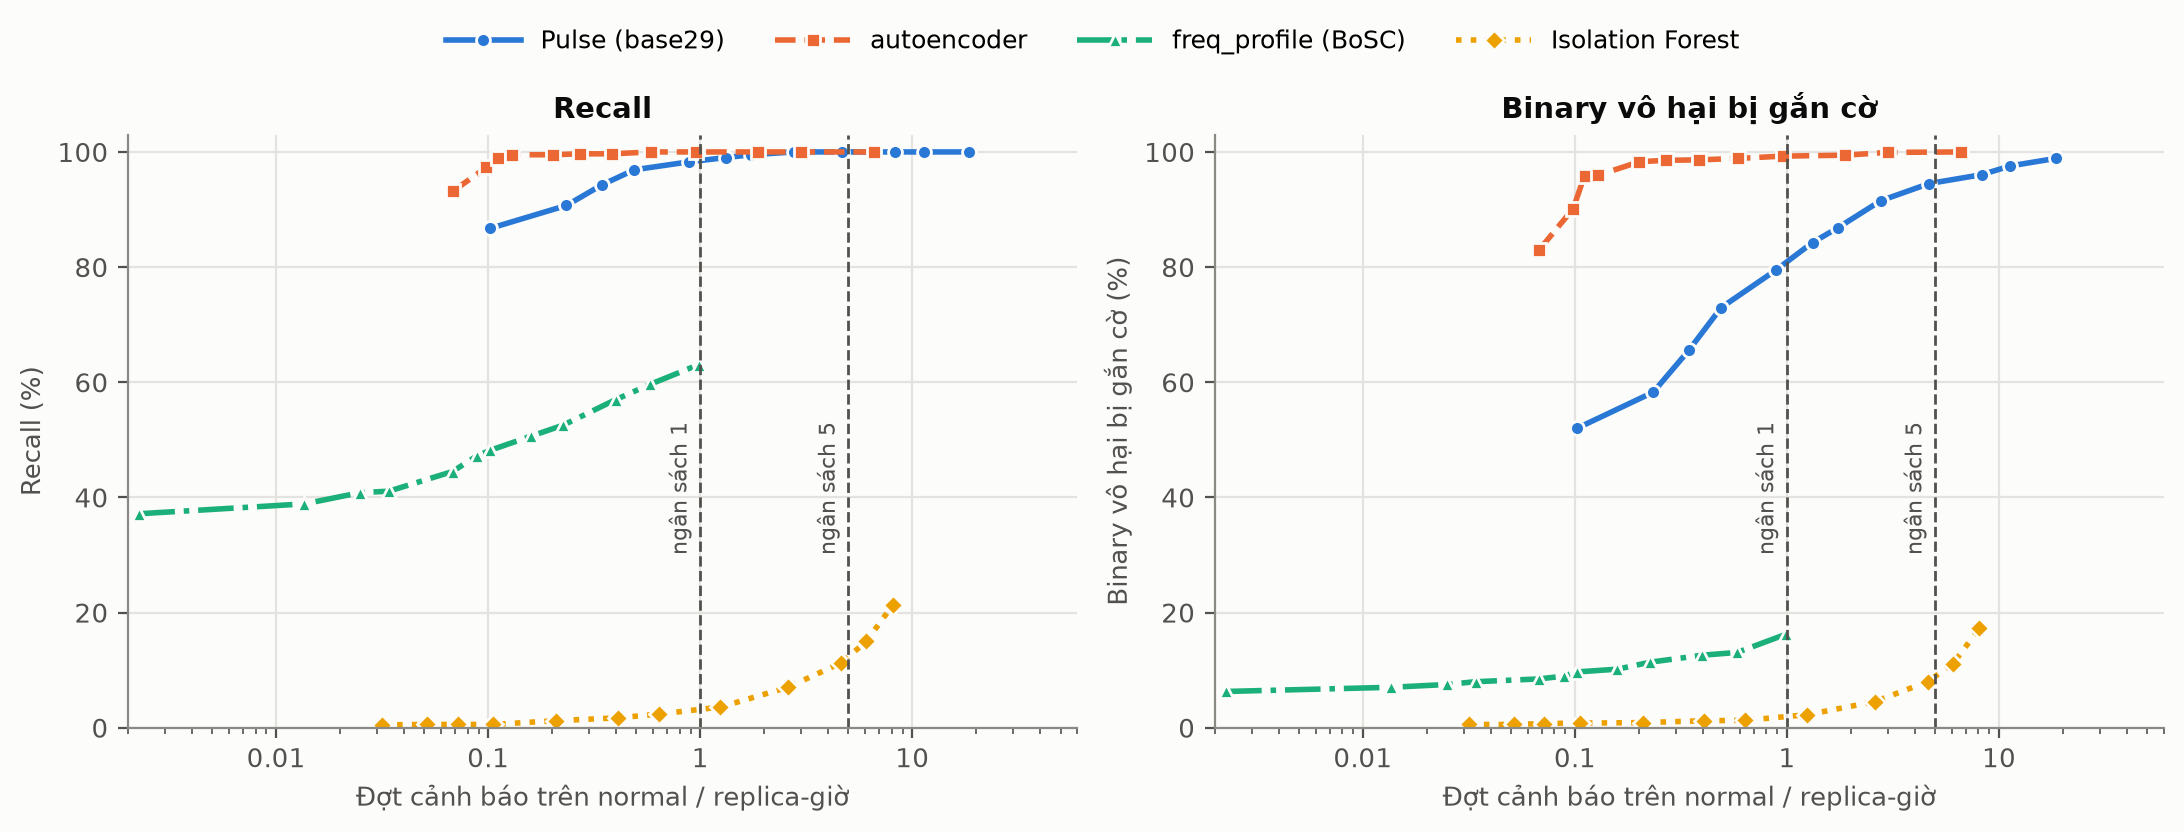
\includegraphics[width=\linewidth]{baselines-budget.png}
  \caption{Recall và tỉ lệ binary vô hại bị gắn cờ theo gánh cảnh báo, Pulse so với ba baseline; mỗi điểm là một hệ số α (development).}
  \label{fig:baselines-budget}
\end{figure}

\section{Đường tới người nhận cảnh báo}

Preview trong decision chưa phải là lúc người vận hành biết. Ở lượt cuối, đường push qua Alertmanager cho 497/525 trial ở mọi tốc độ, tính từ sự kiện kernel tới lúc Alertmanager nhận:

\begin{itemize}
\tightlist
\item
  p50 0,61 s, p95 2,31 s;
\item
  lượt trước, chỉ có ML: p95 3,91 s.
\end{itemize}

Đường Prometheus chuẩn, kéo theo chu kỳ, chậm hơn nhiều: ngay cả với chu kỳ kéo nhanh, p50 đã là 6,4 s. Vì vậy bridge đẩy thẳng là lựa chọn đúng cho mục tiêu dưới 3 s.

\begin{figure}[htbp]
  \centering
  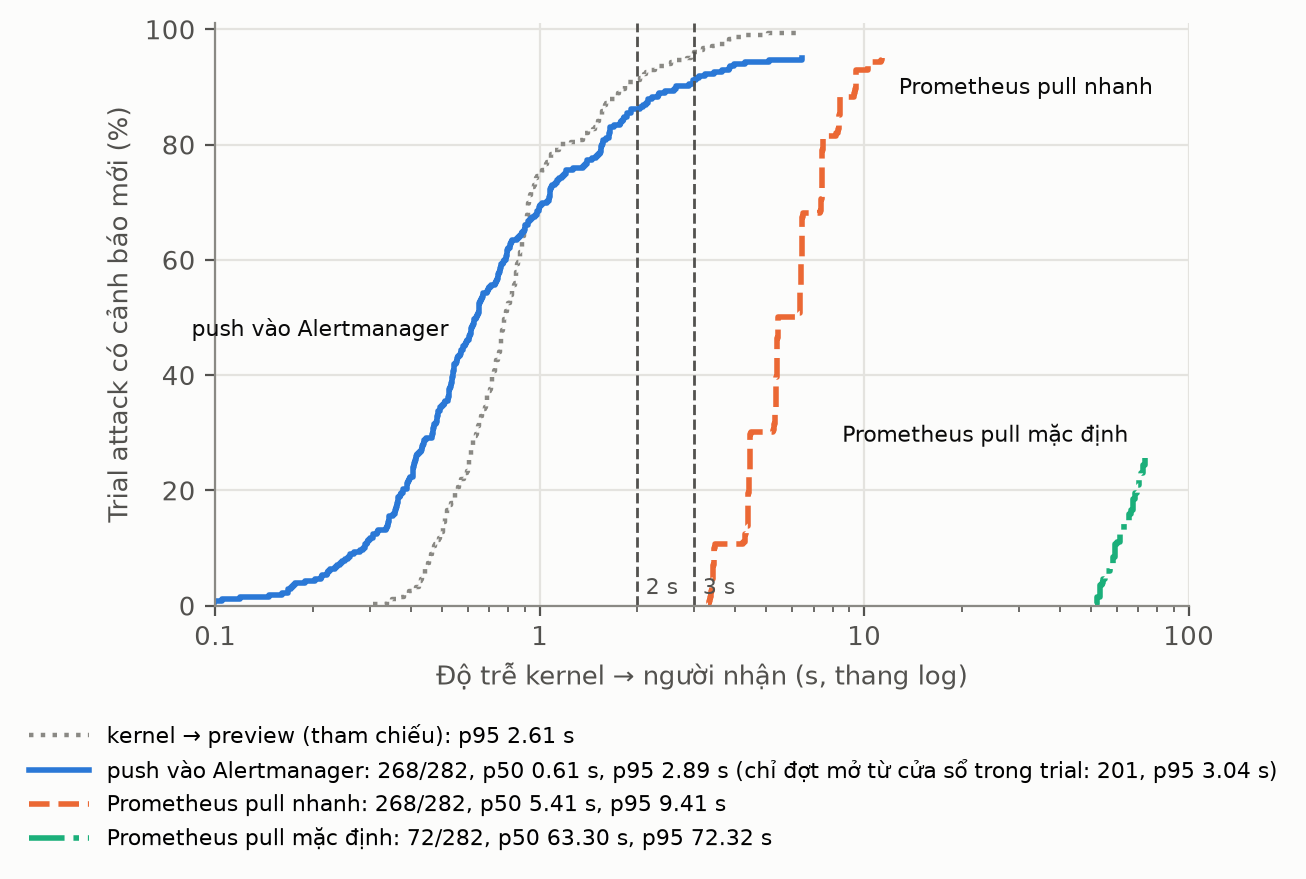
\includegraphics[width=\linewidth]{alert-delivery-cdf.png}
  \caption{Độ trễ kernel → người nhận theo từng đường cảnh báo trên lượt \texttt{pulse-\allowbreak{}stable-\allowbreak{}confirm}: push vào Alertmanager, Prometheus pull nhanh và mặc định.}
  \label{fig:alert-delivery-cdf}
\end{figure}

\section{RQ3: gánh cảnh báo}

Gánh cảnh báo giảm từ 6,74 đợt/replica-giờ xuống 1,50 mà recall vẫn ≥ 95\%, nhưng vẫn gấp khoảng 15 lần ngân sách 0,1. Bốn hướng đã được thử theo protocol đăng ký trước:

\begin{enumerate}
\def\labelenumi{\arabic{enumi}.}
\tightlist
\item
  \textbf{Chỉnh luật dừng (CUSUM, lưới 58 chính sách)} đánh đổi gánh với độ trễ đúng như lý thuyết: siết tham số đưa control về 0,6--2\% nhưng p95 lên 3--5 s.
\item
  \textbf{Chiến lược calibration từ tài liệu} (NexCP, ACI, Mondrian theo node, làm mới theo chu kỳ):

  \begin{itemize}
  \tightlist
  \item
    trên dữ liệu mới, trong 24 giờ sau một lần làm mới, không chiến lược nào thắng;
  \item
    trên soak 48 giờ với calibration đã cũ, làm mới mỗi giờ trên 12 giờ trước giảm 37\% gánh mà không mất recall (development).
  \end{itemize}
\item
  \textbf{Chiết khấu theo replica} đạt test blind (1,74 đợt/replica-giờ, control 2,9\%), rồi được xác nhận live (1,69, bằng 0,37 lần CUSUM).
\item
  \textbf{Lọc probe} giảm gánh nhưng làm chậm đường cảnh báo (mục 6.6).
\end{enumerate}

Cảnh báo còn lại chủ yếu là \emph{benign trigger}:

\begin{itemize}
\tightlist
\item
  57,9\% case trên normal trùng lúc có exec, phần lớn là probe exec của Kubernetes;
\item
  một replica Kafka lệch hệ thống so với hai broker kia và là nguồn gánh lớn nhất.
\end{itemize}

Calibration tự làm mới trong worker (mục~\ref{sec:live-recal}) đã qua smoke với kiểm cài đặt khớp 100\%; lượt xác nhận 24 giờ đang chạy (29--30/10), kết quả sẽ được bổ sung. Lượt này loại khoảng campaign khỏi calibration như bản offline; đây là một giới hạn, vì hệ thống vận hành thật không biết lúc nào bị tấn công.

\begin{figure}[htbp]
  \centering
  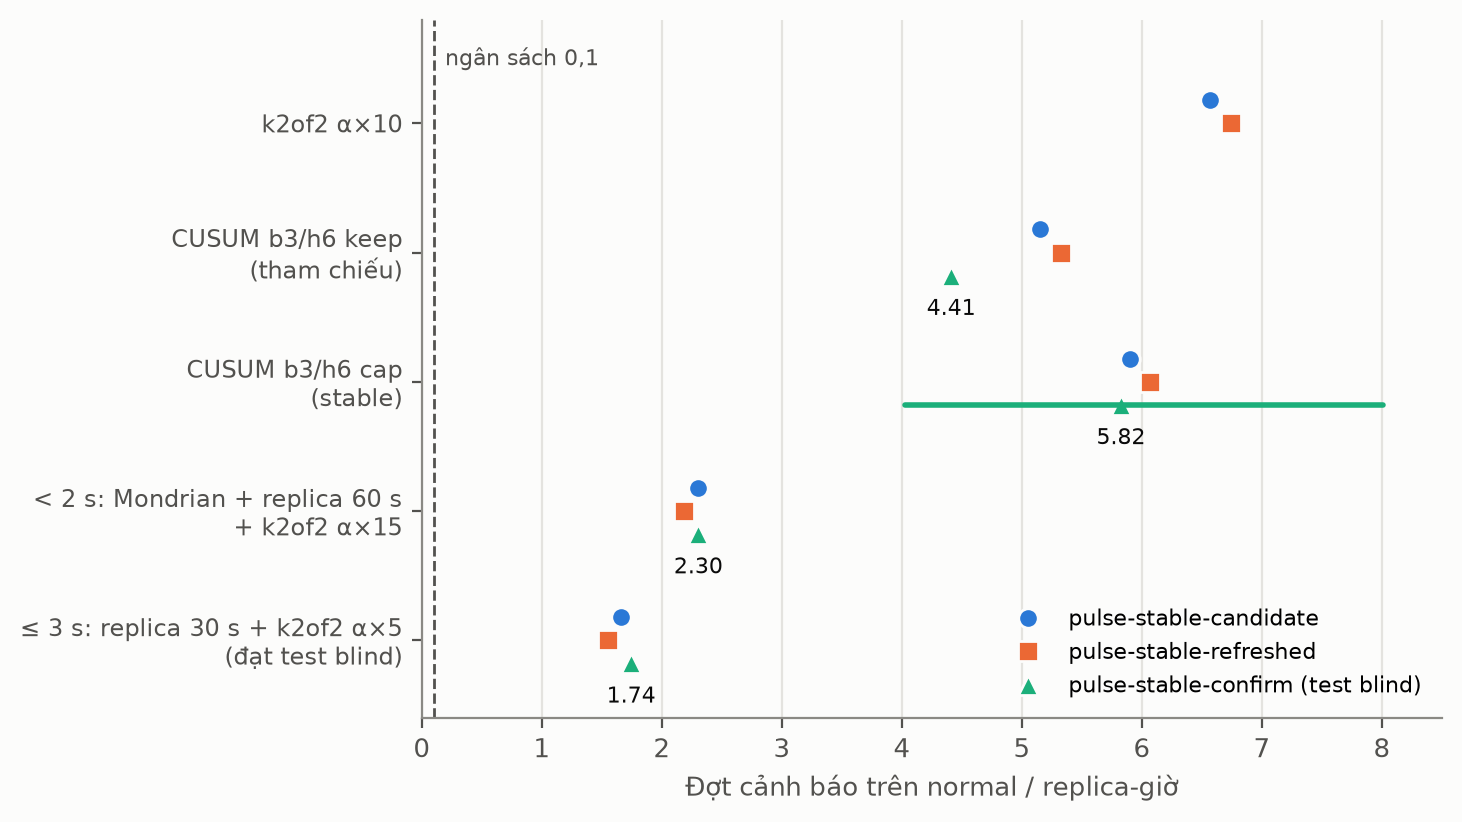
\includegraphics[width=\linewidth]{burden-levers.png}
  \caption{Gánh cảnh báo trên normal (đợt/replica-giờ) của các cấu hình giảm gánh trên hai lượt development và test blind, kèm ngân sách 0,1.}
  \label{fig:burden-levers}
\end{figure}

\section{RQ5: truy nguyên nguyên nhân}

\begingroup\small
\begin{longtable}[]{@{}>{\raggedright\arraybackslash}p{\dimexpr 0.249\linewidth-2\tabcolsep\relax}>{\raggedright\arraybackslash}p{\dimexpr 0.195\linewidth-2\tabcolsep\relax}>{\raggedright\arraybackslash}p{\dimexpr 0.221\linewidth-2\tabcolsep\relax}>{\raggedright\arraybackslash}p{\dimexpr 0.149\linewidth-2\tabcolsep\relax}>{\raggedright\arraybackslash}p{\dimexpr 0.186\linewidth-2\tabcolsep\relax}@{}}
\toprule\noalign{}
Lượt & Tấn công có case riêng & Gộp sau case binary vô hại & Top-1 / top-3 & Cảnh báo → case p95 (s) \\
\midrule\noalign{}
\endhead
\bottomrule\noalign{}
\endlastfoot
pulse-\allowbreak{}stable-\allowbreak{}candidate & 86,7\% (273/315) & 31 & 99,6\% / 99,6\% & 2,52 \\
pulse-\allowbreak{}stable-\allowbreak{}refreshed & 86,7\% (273/315) & 37 & 100\% / 100\% & 2,52 \\
pulse-\allowbreak{}stable-\allowbreak{}confirm & 86,9\% (456/525) & 56 & 99,8\% / 99,8\% & 2,50 \\
pulse-\allowbreak{}peer-\allowbreak{}discount-\allowbreak{}confirm & 87,6\% (459/524) & 44 & 99,8\% / 100\% & 2,59 \\
pulse-\allowbreak{}final-\allowbreak{}system-\allowbreak{}confirm & 89,3\% (469/525) & 40 & 14,1\% / 100\% & 2,67 \\
\end{longtable}
\endgroup

Top-1 là tỉ lệ case có binary tấn công đứng hạng 1 trong danh sách nghi phạm. Top-1 của 4 lượt đầu bị thổi phồng, vì binary vô hại và binary tấn công dùng chung một đường dẫn. Khi binary vô hại có tên riêng ở lượt cuối, nó thường đứng hạng 1 và binary tấn công đứng hạng 2--3:

\begin{itemize}
\tightlist
\item
  top-1 còn 14,1\%, top-3 vẫn 100\%;
\item
  nguyên nhân là luật phá hoà: hai binary thường bằng điểm (6 = binary mới + exec trong cửa sổ), và khi hoà, luật cũ xếp theo thứ tự bảng chữ cái của đường dẫn, nên \texttt{sentinel-\allowbreak{}benign-\allowbreak{}exec-\allowbreak{}control} luôn đứng trước \texttt{sentinel-\allowbreak{}runtime-\allowbreak{}attack-\allowbreak{}blind};
\item
  khi hoà mà xếp process khởi chạy gần cảnh báo nhất lên trước, top-1 trên chính lượt này lên 100\% (469/469). Đây là kết quả development; kiểm blind đã được đăng ký trên lượt kế tiếp. Trong campaign, binary vô hại luôn chạy trước tấn công 15 s, nên luật mới thắng một phần nhờ thiết kế campaign; nó chỉ chứng minh luật cũ là artifact, chưa chứng minh luật mới tốt trong mọi trường hợp.
\end{itemize}

Với 40 tấn công không có case riêng ở lượt cuối, nguyên nhân được quy cho từng bước:

\begin{itemize}
\tightlist
\item
  25 bị từ chối ở bước kiểm exec của case tiếp nối;
\item
  8 không có đợt cảnh báo mới;
\item
  5 có cảnh báo tới chưa đủ 10 s sau case trước;
\item
  2 nằm trong đợt cảnh báo của binary vô hại kéo dài sang.
\end{itemize}

Giả thuyết cho nhóm lớn nhất: khi cảnh báo tới, sự kiện exec của tấn công chưa vào nhật ký exec. Giả thuyết này chưa được kiểm chứng.

\section{RQ6: chi phí}

\textbf{Microbenchmark syscall} trên một worker, ba điều kiện luân phiên, 5 vòng:

\begin{longtable}[]{@{}>{\raggedright\arraybackslash}p{\dimexpr 0.152\linewidth-2\tabcolsep\relax}>{\raggedright\arraybackslash}p{\dimexpr 0.237\linewidth-2\tabcolsep\relax}>{\raggedright\arraybackslash}p{\dimexpr 0.403\linewidth-2\tabcolsep\relax}>{\raggedright\arraybackslash}p{\dimexpr 0.207\linewidth-2\tabcolsep\relax}@{}}
\toprule\noalign{}
Syscall & ns/op khi không có probe & Thêm khi container được theo dõi {[}CI 95\%{]} & ns thêm mỗi syscall \\
\midrule\noalign{}
\endhead
\bottomrule\noalign{}
\endlastfoot
\texttt{getpid} & 1.069 & +24,0\% {[}+17,0; +31,1{]} & \textasciitilde250 \\
\texttt{read} 4 KB & 1.531 & +16,7\% {[}+11,2; +19,2{]} & \textasciitilde253 \\
\texttt{open} + \texttt{close} & 8.134 & +9,4\% {[}+4,6; +17,0{]} & \textasciitilde451 (2 syscall) \\
\texttt{mmap} + \texttt{munmap} & 11.378 & +8,8\% {[}+1,3; +10,5{]} & \textasciitilde400 (2 syscall) \\
\end{longtable}

\begin{itemize}
\tightlist
\item
  Container \textbf{không} được theo dõi vẫn trả khoảng 80--230 ns, vì probe gắn vào \texttt{sys\_\allowbreak{}enter} của cả node rồi mới lọc theo cgroup.
\item
  Mốc không có probe đã cao (\texttt{getpid} khoảng 1,07 µs), nhiều khả năng do VM và các probe khác của cụm. Vì vậy số ns tuyệt đối mới là số so sánh được, không phải phần trăm.
\item
  Worker chấm điểm dùng 13--31\% một core mỗi node.
\end{itemize}

\textbf{Độ trễ request của ứng dụng thật.} Probe làm p95 của request tăng khoảng 3--8\%, nhưng khoảng tin cậy rộng, nên luận văn không nói được rằng mức tăng dưới 5\%. Phép đo theo protocol \texttt{app-\allowbreak{}overhead-\allowbreak{}v1} (cùng amendment 1), đăng ký trước khi đo, chạy ngày 29/10 từ 09:52 đến 11:56:

\begin{itemize}
\tightlist
\item
  hai điều kiện xen kẽ trên cả ba worker: không có probe, và probe của hệ thống cuối gắn đúng như khi live (mọi container \texttt{production} được theo dõi);
\item
  12 vòng, mỗi vòng một block 300 s cho mỗi điều kiện, thứ tự đảo ở vòng chẵn; 30 s đầu của block bị bỏ;
\item
  client mở chạy trên master, 8 request/s, không chờ phản hồi trước; bốn endpoint gọi lần lượt qua ingress Istio, đúng đường người dùng đi; tải normal của AIMS vẫn chạy;
\item
  chỉ số chính: tỉ lệ p95 có probe / không probe của từng endpoint, ghép cặp theo vòng; trung vị qua 12 vòng, CI bootstrap 95\% theo vòng.
\end{itemize}

\begin{longtable}[]{@{}>{\raggedright\arraybackslash}p{\dimexpr 0.25\linewidth-2\tabcolsep\relax}>{\raggedright\arraybackslash}p{\dimexpr 0.19\linewidth-2\tabcolsep\relax}>{\raggedright\arraybackslash}p{\dimexpr 0.19\linewidth-2\tabcolsep\relax}>{\raggedright\arraybackslash}p{\dimexpr 0.2\linewidth-2\tabcolsep\relax}>{\raggedright\arraybackslash}p{\dimexpr 0.17\linewidth-2\tabcolsep\relax}@{}}
\caption{Độ trễ request của AIMS khi có và không có probe (12 vòng, mỗi điều kiện 25.920 request).}\\
\toprule\noalign{}
Endpoint & p95 không probe / có probe (ms) & Thay đổi p95 [CI 95\%] & Thay đổi p50 [CI 95\%] & p50 thêm (ms) \\
\midrule\noalign{}
\endhead
\bottomrule\noalign{}
\endlastfoot
\texttt{/} & 11,5 / 12,1 & +5,9\% [−1,4; +14,5] & +0,5\% [−0,8; +3,2] & 0,04 \\
\texttt{/api/\allowbreak{}health/} & 25,1 / 24,3 & +3,2\% [−8,1; +21,2] & +2,0\% [+0,2; +4,4] & 0,14 \\
\texttt{/api/\allowbreak{}products/} & 306,4 / 318,2 & +8,2\% [+0,7; +18,3] & +3,0\% [+1,2; +4,3] & 5,9 \\
\texttt{/api/\allowbreak{}products/\allowbreak{}?page=1} & 309,3 / 320,4 & +5,8\% [+1,4; +17,9] & +2,6\% [+0,4; +5,2] & 5,3 \\
\end{longtable}

Cột p95 là trung vị qua các vòng của p95 từng block; cột thay đổi là trung vị của tỉ lệ ghép cặp, nên hai cột không suy ra nhau trực tiếp (ở \texttt{/api/\allowbreak{}health/}, trung vị p95 giảm nhưng trung vị tỉ lệ tăng).

\begin{itemize}
\tightlist
\item
  \textbf{Theo luật đã đăng ký,} chỉ được nói ``dưới 5\%'' khi cận trên CI dưới +5\% ở cả bốn endpoint. Cận trên thực tế là +14,5\% đến +21,2\%, nên kết luận ``dưới 5\%'' \emph{không} được đưa ra.
\item
  \textbf{Ở trung vị,} p50 tăng 0,5--3,0\%. Hai lệnh đọc \texttt{/api/\allowbreak{}products/} đi qua nhiều service và cơ sở dữ liệu, nên chậm thêm nhiều nhất: khoảng 5--6 ms ở p50 trên nền khoảng 200 ms. Đây là đường có nhiều syscall nhất trong bốn endpoint, nên hướng của kết quả khớp với chi phí theo từng syscall của microbenchmark.
\item
  \textbf{CPU:} tiến trình loader dùng 0,016--0,041 core mỗi worker. Tính cả phần chạy trong kernel, tỉ lệ CPU bận của node tăng 0,4--0,9 điểm phần trăm, tức khoảng 0,09--0,21 core trên 24 core.
\item
  \textbf{Lỗi:} 0,57\% request lỗi khi không có probe và 0,55\% khi có probe. Phần lớn số lỗi rơi vào một đợt timeout khoảng 60 s ở block đầu tiên, khi chưa gắn probe.
\item
  \textbf{Giới hạn:} phép đo chỉ gồm probe trong kernel và việc đọc map. Scorer ở user space không xen kẽ được theo block 5 phút, vì mỗi lần khởi động cần 90 phút pha chọn; CPU của nó được lấy từ các lượt live (13--31\% một core). Phép đo chạy trên một cụm VM, một kernel.
\end{itemize}

\section{LID-DS 2021}

Trên 15 kịch bản lỗ hổng thật của LID-DS 2021, hệ thống cuối phát hiện 77,3\% bản ghi tấn công và báo nhầm trên 3,0\% bản ghi normal, với mọi tham số lấy nguyên từ hệ thống live. STIDE phát hiện mọi bản ghi tấn công, nhưng báo nhầm trên 60,8\% bản ghi normal.

Đánh giá theo protocol \texttt{lidds-\allowbreak{}evaluation-\allowbreak{}v1}, đăng ký ngày 29/10 lúc 09:17, trước mọi lần fit:

\begin{itemize}
\tightlist
\item
  mỗi kịch bản là một workload; model được fit trên training, hiệu chỉnh trên validation và chỉ đánh giá trên hai tập test, đúng cách chia của dataset;
\item
  trace syscall được chuyển thành đúng các frame mà loader eBPF sinh ra, rồi chạy qua cùng bộ dựng 249 feature;
\item
  quyết định giống live nhưng không có chiết khấu theo replica, vì một bản ghi chỉ có một container;
\item
  một bản ghi tấn công được tính là phát hiện khi có cảnh báo kết thúc sau thời điểm exploit đầu tiên mà LID-DS ghi lại; độ trễ tính từ thời điểm đó; bản ghi normal bị báo nhầm khi có bất kỳ cảnh báo nào;
\item
  baseline STIDE \citep{forrest1996}: cơ sở dữ liệu chuỗi 7 tên syscall theo từng thread trên training; một cửa sổ báo khi có chuỗi không có trong cơ sở dữ liệu; không chỉnh tham số.
\end{itemize}

\begin{longtable}[]{@{}>{\raggedright\arraybackslash}p{\dimexpr 0.25\linewidth-2\tabcolsep\relax}>{\raggedright\arraybackslash}p{\dimexpr 0.24\linewidth-2\tabcolsep\relax}>{\raggedright\arraybackslash}p{\dimexpr 0.24\linewidth-2\tabcolsep\relax}>{\raggedright\arraybackslash}p{\dimexpr 0.12\linewidth-2\tabcolsep\relax}>{\raggedright\arraybackslash}p{\dimexpr 0.15\linewidth-2\tabcolsep\relax}@{}}
\caption{LID-DS 2021, gộp 15 kịch bản: 1.815 bản ghi tấn công, 11.341 bản ghi normal (137,5 giờ normal).}\\
\toprule\noalign{}
Nhánh & Phát hiện [CI 95\%] & Bản ghi normal bị báo nhầm [CI 95\%] & Đợt/giờ normal & Độ trễ p50 / p95 (s) \\
\midrule\noalign{}
\endhead
\bottomrule\noalign{}
\endlastfoot
ML & 63,6\% (1154/1815) [61,3; 65,8] & 2,9\% (333/11341) [2,6; 3,3] & 2,46 & 1,33 / 4,13 \\
Tripwire & 63,5\% (1153/1815) [61,3; 65,7] & 0,1\% (7/11341) [0,0; 0,1] & 0,05 & 0,79 / 2,94 \\
Hệ thống (ML hoặc tripwire) & 77,3\% (1403/1815) [75,3; 79,2] & 3,0\% (336/11341) [2,7; 3,3] & 2,48 & 0,77 / 2,71 \\
STIDE & 100,0\% (1815/1815) [99,8; 100,0] & 60,8\% (6899/11341) [59,9; 61,7] & 59,95 & 0,37 / 1,44 \\
\end{longtable}

Hiệu gộp, bootstrap theo kịch bản (10.000 lần), tính bằng điểm phần trăm:

\begin{itemize}
\tightlist
\item
  hệ thống so với ML: phát hiện +13,7 [+0,2; +30,0], báo nhầm +0,0 [+0,0; +0,1];
\item
  hệ thống so với STIDE: phát hiện -22,7 [-42,1; -6,5], báo nhầm -57,9 [-76,6; -38,9].
\end{itemize}

\begingroup\small
\begin{longtable}[]{@{}>{\raggedright\arraybackslash}p{\dimexpr 0.27\linewidth-2\tabcolsep\relax}>{\raggedright\arraybackslash}p{\dimexpr 0.11\linewidth-2\tabcolsep\relax}>{\raggedright\arraybackslash}p{\dimexpr 0.13\linewidth-2\tabcolsep\relax}>{\raggedright\arraybackslash}p{\dimexpr 0.13\linewidth-2\tabcolsep\relax}>{\raggedright\arraybackslash}p{\dimexpr 0.2\linewidth-2\tabcolsep\relax}>{\raggedright\arraybackslash}p{\dimexpr 0.16\linewidth-2\tabcolsep\relax}@{}}
\caption{LID-DS 2021 theo kịch bản (\%). Báo nhầm là tỉ lệ bản ghi normal có cảnh báo.}\\
\toprule\noalign{}
Kịch bản & ML phát hiện & Tripwire phát hiện & Hệ thống phát hiện & Báo nhầm: hệ thống / STIDE & STIDE phát hiện \\
\midrule\noalign{}
\endhead
\bottomrule\noalign{}
\endlastfoot
\texttt{Bruteforce\_CWE-\allowbreak{}307} & 96,4 & 0,0 & 96,4 & 2,7 / 10,7 & 100,0 \\
\texttt{CVE-\allowbreak{}2012-\allowbreak{}2122} & 100,0 & 100,0 & 100,0 & 1,0 / 36,4 & 100,0 \\
\texttt{CVE-\allowbreak{}2014-\allowbreak{}0160} & 5,8 & 0,0 & 5,8 & 15,6 / 3,0 & 100,0 \\
\texttt{CVE-\allowbreak{}2017-\allowbreak{}12635\_6} & 100,0 & 100,0 & 100,0 & 2,1 / 100,0 & 100,0 \\
\texttt{CVE-\allowbreak{}2017-\allowbreak{}7529} & 69,7 & 0,0 & 69,7 & 1,6 / 15,2 & 100,0 \\
\texttt{CVE-\allowbreak{}2018-\allowbreak{}3760} & 4,1 & 100,0 & 100,0 & 2,6 / 98,6 & 100,0 \\
\texttt{CVE-\allowbreak{}2019-\allowbreak{}5418} & 16,7 & 0,0 & 16,7 & 0,7 / 96,8 & 100,0 \\
\texttt{CVE-\allowbreak{}2020-\allowbreak{}13942} & 98,3 & 100,0 & 100,0 & 1,1 / 99,7 & 100,0 \\
\texttt{CVE-\allowbreak{}2020-\allowbreak{}23839} & 51,7 & 100,0 & 100,0 & 2,5 / 39,7 & 100,0 \\
\texttt{CVE-\allowbreak{}2020-\allowbreak{}9484} & 100,0 & 100,0 & 100,0 & 2,4 / 98,8 & 100,0 \\
\texttt{CWE-\allowbreak{}89-\allowbreak{}SQL-\allowbreak{}injection} & 100,0 & 100,0 & 100,0 & 2,0 / 47,1 & 100,0 \\
\texttt{EPS\_CWE-\allowbreak{}434} & 100,0 & 100,0 & 100,0 & 2,1 / 37,5 & 100,0 \\
\texttt{Juice-\allowbreak{}Shop} & 4,1 & 62,0 & 63,6 & 0,8 / 99,9 & 100,0 \\
\texttt{PHP\_CWE-\allowbreak{}434} & 100,0 & 100,0 & 100,0 & 1,4 / 31,4 & 100,0 \\
\texttt{ZipSlip} & 3,4 & 0,0 & 3,4 & 5,8 / 97,8 & 100,0 \\
\end{longtable}
\endgroup

\begin{itemize}
\tightlist
\item
  \textbf{Mạnh:} hệ thống phát hiện 100\% ở 9/15 kịch bản, với 1,0--2,6\% bản ghi normal bị báo nhầm. Tripwire phát hiện 100\% ở 9 kịch bản và gần như không báo nhầm (0,1\% gộp). Nó bù cho ML ở chỗ ML yếu, ví dụ \texttt{CVE-\allowbreak{}2018-\allowbreak{}3760}: ML 4,1\%, tripwire 100\%.
\item
  \textbf{Yếu:} \texttt{CVE-\allowbreak{}2014-\allowbreak{}0160} (Heartbleed, 5,8\%), \texttt{ZipSlip} (3,4\%), \texttt{CVE-\allowbreak{}2019-\allowbreak{}5418} (16,7\%), \texttt{Juice-\allowbreak{}Shop} (63,6\%, gần như chỉ nhờ tripwire) và \texttt{CVE-\allowbreak{}2017-\allowbreak{}7529} (69,7\%). Ở các kịch bản này, exploit chạy bên trong chính process của dịch vụ. Cách giải thích khả dĩ là exploit không cần syscall mới, cũng không đổi đáng kể tần suất syscall; đây là cách giải thích, chưa được kiểm riêng. Nó khớp với giới hạn ở mục~\ref{sec:limits-novelty}: số đếm syscall yếu với tấn công đi qua ứng dụng.
\item
  \textbf{STIDE} \emph{bắt} mọi bản ghi tấn công, nhưng đổi lại báo nhầm trên 60,8\% bản ghi normal (gần 60 đợt mỗi giờ normal). Biến thể \emph{any-mismatch} không có ngưỡng, và protocol không cho chỉnh tham số sau khi xem kết quả. Vì vậy con số này là của STIDE nguyên bản, không phải của một STIDE đã tinh chỉnh.
\item
  \textbf{Độ trễ:} p95 2,71 s của hệ thống tính từ thời điểm exploit đến cuối cửa sổ cảnh báo, trong điều kiện replay; chưa gồm đường tới người nhận.
\item
  \textbf{Giới hạn đã phát hiện sau khi chạy:} bộ chuyển đổi đã bỏ bốn syscall thật vì sysdig ghi tên khác với bảng ABI: \texttt{pread}, \texttt{pwrite}, \texttt{sigreturn}, \texttt{prlimit}. Tổng cộng khoảng 15 triệu lượt gọi ở 12/15 kịch bản. Lỗi này giống nhau giữa train và test nên không làm rò nhãn, nhưng Pulse thấy ít thông tin hơn STIDE (STIDE đọc tên thô). Bộ chuyển đổi đã được sửa, và một lượt chạy lại đã được đăng ký là phân tích độ nhạy (amendment 1). Bảng trên là kết quả của lượt đã đăng ký.
\item
  \textbf{Đặt cạnh số đã công bố:} kết quả duy nhất trên đủ 15 kịch bản LID-DS 2021 mà tác giả dataset công bố là STIDE (chuỗi 7 syscall, cửa sổ 100 syscall, ngưỡng là điểm cao nhất trên validation), với tỉ lệ phát hiện trung bình 0,59 \citep{grimmer2022}. Hệ thống của luận văn đạt 0,773. Báo nhầm của bài đó được đếm theo số cụm báo động chứ không theo bản ghi, nên chỉ so được tỉ lệ phát hiện. LID-DS chưa có ngưỡng đạt nào được đăng ký.
\item
  \textbf{Lượt v2 đã đăng ký} (protocol \texttt{lidds-\allowbreak{}evaluation-\allowbreak{}v2}): thêm các tín hiệu theo tham số và giá trị trả về (đường dẫn mới, lỗi theo errno, số byte) và chuỗi syscall theo thread, với ngưỡng là điểm cao nhất trên validation. Protocol ghi rõ thiết kế được làm sau khi đã thấy kết quả trên, nên bằng chứng độc lập chỉ đến từ lượt xác nhận trên LID-DS 2019 và CB-DS.
\end{itemize}
